\documentclass[12pt]{article}
 
\usepackage[margin=1in]{geometry}
\usepackage{amsmath,amsthm,amssymb}
\usepackage{mathtools}
\DeclarePairedDelimiter{\ceil}{\lceil}{\rceil}
%\usepackage{mathptmx}
\usepackage{accents}
\usepackage{comment}
\usepackage{graphicx}
\usepackage{IEEEtrantools}
 \usepackage{float}
 
\newcommand{\N}{\mathbb{N}}
\newcommand{\Z}{\mathbb{Z}}
\newcommand{\R}{\mathbb{R}}
\newcommand{\Q}{\mathbb{Q}}
\newcommand*\conj[1]{\bar{#1}}
\newcommand*\mean[1]{\bar{#1}}
\newcommand\widebar[1]{\mathop{\overline{#1}}}


\newcommand{\cc}{{\mathbb C}}
\newcommand{\rr}{{\mathbb R}}
\newcommand{\qq}{{\mathbb Q}}
\newcommand{\nn}{\mathbb N}
\newcommand{\zz}{\mathbb Z}
\newcommand{\aaa}{{\mathcal A}}
\newcommand{\bbb}{{\mathcal B}}
\newcommand{\rrr}{{\mathcal R}}
\newcommand{\fff}{{\mathcal F}}
\newcommand{\ppp}{{\mathcal P}}
\newcommand{\eps}{\varepsilon}
\newcommand{\vv}{{\mathbf v}}
\newcommand{\ww}{{\mathbf w}}
\newcommand{\xx}{{\mathbf x}}
\newcommand{\ds}{\displaystyle}
\newcommand{\Om}{\Omega}
\newcommand{\dd}{\mathop{}\,\mathrm{d}}
\newcommand{\ud}{\, \mathrm{d}}
\newcommand{\seq}[1]{\left\{#1\right\}_{n=1}^\infty}
\newcommand{\isp}[1]{\quad\text{#1}\quad}
\newcommand*\diff{\mathop{}\!\mathrm{d}}

\DeclareMathOperator{\imag}{Im}
\DeclareMathOperator{\re}{Re}
\DeclareMathOperator{\diam}{diam}
\DeclareMathOperator{\Tr}{Tr}
\DeclareMathOperator{\cis}{cis}

\def\upint{\mathchoice%
    {\mkern13mu\overline{\vphantom{\intop}\mkern7mu}\mkern-20mu}%
    {\mkern7mu\overline{\vphantom{\intop}\mkern7mu}\mkern-14mu}%
    {\mkern7mu\overline{\vphantom{\intop}\mkern7mu}\mkern-14mu}%
    {\mkern7mu\overline{\vphantom{\intop}\mkern7mu}\mkern-14mu}%
  \int}
\def\lowint{\mkern3mu\underline{\vphantom{\intop}\mkern7mu}\mkern-10mu\int}




\newenvironment{theorem}[2][Theorem]{\begin{trivlist}
\item[\hskip \labelsep {\bfseries #1}\hskip \labelsep {\bfseries #2.}]}{\end{trivlist}}
\newenvironment{lemma}[2][Lemma]{\begin{trivlist}
\item[\hskip \labelsep {\bfseries #1}\hskip \labelsep {\bfseries #2.}]}{\end{trivlist}}
\newenvironment{exercise}[2][Exercise]{\begin{trivlist}
\item[\hskip \labelsep {\bfseries #1}\hskip \labelsep {\bfseries #2.}]}{\end{trivlist}}
\newenvironment{problem}[2][Problem]{\begin{trivlist}
\item[\hskip \labelsep {\bfseries #1}\hskip \labelsep {\bfseries #2.}]}{\end{trivlist}}
\newenvironment{question}[2][Question]{\begin{trivlist}
\item[\hskip \labelsep {\bfseries #1}\hskip \labelsep {\bfseries #2.}]}{\end{trivlist}}
\newenvironment{corollary}[2][Corollary]{\begin{trivlist}
\item[\hskip \labelsep {\bfseries #1}\hskip \labelsep {\bfseries #2.}]}{\end{trivlist}}

\newenvironment{solution}{\begin{proof}[Solution]}{\end{proof}}
 
\begin{document}
 
% --------------------------------------------------------------
%                         Start here
% --------------------------------------------------------------
\title{Math 122B Homework 3}
\author{Ethan Martirosyan}
\date{\today}
\maketitle
\hbadness=99999
\hfuzz=50pt
\section*{Chapter 11}
\subsection*{Problem 1}
\subsubsection*{Part A}
Since $\deg (1+x^2)^2 - \deg x^2 \geq 2$, we have
\[
\int_{-\infty}^\infty \frac{x^2}{(1+x^2)^2} \diff x = 2\pi i \cdot \text{Res}\bigg(\frac{z^2}{(1+z^2)^2}; i\bigg) 
\] since $i$ is the only root in the upper half plane. To find the residue, we first compute
\[
(z-i)^2 \cdot \frac{z^2}{(1+z^2)^2} = (z-i)^2 \cdot \frac{z^2}{(z+i)^2(z-i)^2} = \frac{z^2}{(z+i)^2}
\] Then we differentiate:
\[
\frac{\diff}{\diff z} \frac{z^2}{(z+i)^2} = \frac{2iz}{(z+i)^3}
\] Evaluating at $i$, we obtain
\[
\text{Res}\bigg(\frac{z^2}{(1+z^2)^2}; i\bigg)  = \frac{2i(i)}{(i+i)^3} = \frac{-2}{-8i} = \frac{1}{4i}
\] so that
\[
\int_{-\infty}^\infty \frac{x^2}{(1+x^2)^2} \diff x = 2\pi i \cdot \text{Res}\bigg(\frac{z^2}{(1+z^2)^2}; i\bigg) = \frac{\pi}{2} 
\]
\subsubsection*{Part B}
Since $\deg (x^2+4)^2 (x^2 + 9) - \deg x^2  \geq 2$, we know that this integral must converge. Furthermore, since the function is even, we have
\[
\int_0^\infty \frac{x^2}{(x^2+4)^2 (x^2 + 9)} \diff x = \frac{1}{2} \int_{-\infty}^\infty \frac{x^2}{(x^2+4)^2 (x^2 + 9)} \diff x
\] The only singularities of this function in the upper half plane are at $2i$ and $3i$. First, we compute
\[
\text{Res}\bigg(\frac{z^2}{(z^2+4)^2(z^2+9)}; 2i\bigg)
\] as follows: We multiply the function by $(z-2i)^2$. Then we obtain
\[
(z-2i)^2\cdot \frac{z^2}{(z^2+4)^2(z^2+9)} = \frac{z^2}{(z+2i)^2(z^2+9)}
\] Then, we must differentiate:
\[
\frac{\diff}{\diff z} \frac{z^2}{(z+2i)^2(z^2+9)} = -\frac{2z(z^3 - 18i)}{(z+2i)^3(z^2+9)^2}
\] Substituting $z = 2i$, we obtain
\[
\text{Res}\bigg(\frac{z^2}{(z^2+4)^2(z^2+9)}; 2i\bigg) = -\frac{2(2i)((2i)^3 - 18i)}{(2i+2i)^3((2i)^2+9)^2} = \frac{-104}{-1600i} = -\frac{13}{200}i
\] Next, we compute
\[
\text{Res}\bigg(\frac{z^2}{(z^2+4)^2(z^2+9)}; 3i\bigg)
\] as follows: Let us write 
\[
\frac{z^2}{(z^2+4)^2(z^2+9)} = \frac{z^2}{(z^2+4)^2(z+3i)(z-3i)} = \frac{\frac{z^2}{(z^2+4)^2(z+3i)}}{z-3i}
\] Substituting $z = 3i$ into the numerator yields 
\[
 \text{Res}\bigg(\frac{z^2}{(z^2+4)^2(z^2+9)}; 3i\bigg) = \frac{(3i)^2}{((3i)^2+4)^2(3i+3i)} = \frac{-9}{(-9+4)^2(3i+3i)} = \frac{-9}{150i} = \frac{3}{50}i
\] Finally, we obtain
\begin{align*}
&\int_0^\infty \frac{x^2}{(x^2+4)^2 (x^2 + 9)} \diff x = \frac{1}{2} \int_{-\infty}^\infty \frac{x^2}{(x^2+4)^2 (x^2 + 9)} \diff x \\
& = \pi i \Bigg( \text{Res}\bigg(\frac{z^2}{(z^2+4)^2(z^2+9)}; 2i\bigg) + \text{Res}\bigg(\frac{z^2}{(z^2+4)^2(z^2+9)}; 3i\bigg)\Bigg) \\
&= \pi i\bigg(-\frac{13}{200}i + \frac{3}{50}i\bigg)
\end{align*}
\subsubsection*{Part C}
First, we note that $1/(x^4+x^2+1)$ is even so that
\[
\int_0^\infty \frac{\diff x}{x^4 + x^2 + 1} = \frac{1}{2} \int_{-\infty}^\infty \frac{\diff x}{x^4 + x^2 + 1}
\] We need to find the zeroes of $z^4 + z^2 + 1$ in the upper half plane. Let us make the substitution $w = z^2$. Then we must solve $w^2 + w + 1 = 0$. The solutions of this are $w = e^{2\pi i/3}$ and $w = e^{4 \pi i / 3}$. From this, we get $z = e^{\pi i/3}$ and $z = e^{2\pi i / 3}$. We now compute the residues of $1/(z^4+z^2+1)$ at these two points. We have
\[
\text{Res}\bigg(\frac{1}{z^4+z^2+1}; e^{\pi i /3}\bigg) = \frac{1}{4(e^{\pi i /3})^3 + 2e^{\pi i / 3}} = \frac{1}{-4 + 1 + \sqrt{3}i} = \frac{1}{-3+\sqrt{3}i}
\] and
\[
\text{Res}\bigg(\frac{1}{z^4+z^2+1}; e^{ 2 \pi i /3}\bigg) = \frac{1}{4(e^{2\pi i /3})^3 + 2e^{2\pi i / 3}} = \frac{1}{4 - 1 -\sqrt{3}} = \frac{1}{3+\sqrt{3}i}
\] so that
\[
\int_0^\infty \frac{\diff x}{x^4 + x^2 + 1} = \frac{1}{2} \int_{-\infty}^\infty \frac{\diff x}{x^4 + x^2 + 1} = \pi i \bigg(\frac{1}{-3+\sqrt{3}i} + \frac{1}{3+\sqrt{3}i} \bigg)
\]
\subsubsection*{Part E}
Note that 
\[
\frac{\cos x}{1+x^2}
\] is an even function so that we may write
\[
\int_0^\infty \frac{\cos x}{1+x^2} \diff x = \frac{1}{2} \int_{-\infty}^\infty \frac{\cos x}{1+x^2} \diff x
\] Since the only pole of this function in the upper half plane is $i$, we have
\[
\int_{-\infty}^\infty \frac{\cos x}{1+x^2} \diff x = \re \Bigg[ 2\pi i \cdot \text{Res}\bigg(\frac{e^{iz}}{1+z^2}; i \bigg) \Bigg] = \re\bigg(2\pi i \frac{e^{-1}}{2i}\bigg) = \frac{\pi}{e}
\] Thus we obtain 
\[
\int_0^\infty \frac{\cos x}{1+x^2} \diff x = \frac{1}{2} \int_{-\infty}^\infty \frac{\cos x}{1+x^2} \diff x = \frac{\pi}{2e} 
\]
\subsubsection*{Part F}
First, we note that the residues are at $z = 2e^{\pi i /3}, -2, 2e^{5\pi i / 3}$. We first compute
\[
\text{Res}\bigg(\frac{\log z}{z^3 + 8}; 2e^{\pi i /3}\bigg)
\] To do this, we note that
\[
\frac{\log z}{(z^3+8)^\prime} = \frac{\log z}{3z^2}  
\] so that
\[
\text{Res}\bigg(\frac{\log z}{z^3 + 8}; 2e^{\pi i /3}\bigg) = \frac{\log 2e^{\pi i /3}}{3(2e^{\pi i/3})^2}
\] Similarly, we have
\[
\text{Res}\bigg(\frac{\log z}{z^3 + 8}; 2e^{\pi i}\bigg) = \frac{\log 2e^{\pi i}}{3(2e^{\pi i})^2}
\] We also have
\[
\text{Res}\bigg(\frac{\log z}{z^3 + 8}; 2e^{5 \pi i / 3}\bigg) = \frac{\log 2e^{5 \pi i/3}}{3(2e^{5 \pi i /3})^2}
\] so that the integral is just
\[
-\bigg(\frac{\log 2e^{\pi i /3}}{3(2e^{\pi i/3})^2} + \frac{\log 2e^{\pi i}}{3(2e^{\pi i})^2} + \frac{\log 2e^{5 \pi i/3}}{3(2e^{5 \pi i /3})^2} \bigg)
\]
\newpage
\subsection*{Problem 2}
Let us consider
\[
e^{2iz} - 1 - 2i z = - 1 - 2iz + 1 + 2i z + \frac{(2iz)^2}{2} + \cdots = \frac{(2iz)^2}{2} + \cdots
\] Thus we find that
\[
\frac{e^{2iz} - 1 - 2i z}{z^2}
\] is entire. Therefore, we know that for any closed contour $C_R$ (consisting of the line segment from $-R$ to $R$ and the semi-circle $\Gamma_R$), we have
\[
\int_{C_R} \frac{e^{2iz} - 1 - 2i z}{z^2} \diff z = 0
\] Let us split this integral into the real segment and the semi-circle $\Gamma_R$. Then we have
\[
\int_{-R}^R \frac{e^{2ix} - 1 - 2ix }{x^2} \diff x + \int_{\Gamma_R} \frac{e^{2iz} - 1 - 2i z}{z^2} \diff z = 0
\] Let us consider the integral
\[
 \int_{\Gamma_R} \frac{e^{2iz} - 1 - 2i z}{z^2} \diff z = \int_{\Gamma_R} \frac{e^{2iz} - 1}{z^2} \diff z - 2i\int_{\Gamma_R} \frac{1}{z} \diff z
\] Using reasoning similar to that in the textbook, it can be shown that
\[
\int_{\Gamma_R} \frac{e^{2iz} - 1}{z^2} \diff z \rightarrow 0
\] as $R \rightarrow \infty$. Furthermore, we have
\[
\int_{\Gamma_R} \frac{1}{z} \diff z = \int_{-\pi/2}^{\pi/2} \frac{1}{Re^{i\theta}} \cdot i Re^{i\theta} \diff \theta = i \int_{-\pi/2}^{\pi/2} \diff \theta = i \pi
\] Thus we obtain
\[
\lim_{R\rightarrow \infty}  \int_{\Gamma_R} \frac{e^{2iz} - 1 - 2i z}{z^2} \diff z = 2 \pi
\] so that
\[
 \int_{-\infty}^\infty \frac{e^{2ix} - 1 - 2ix }{x^2} \diff x = -2 \pi
\] Now, we note that
\[
e^{2ix} = (e^{ix})^2 = (\cos x + i \sin x)^2 = \cos^2 x + 2i\sin x \cos x - \sin^2 x = 1 + 2i\sin x \cos x - 2\sin^2 x
\] so that
\[
e^{2ix} - 1 - 2ix = -2\sin^2x + 2i(\sin x \cos x - x)
\] From this, we obtain
\[
 \int_{-\infty}^\infty \frac{e^{2ix} - 1 - 2ix }{x^2} \diff x = -2 \int_{-\infty}^\infty \frac{\sin^2x}{x^2} \diff x  + 2i \int_{-\infty}^\infty \frac{\sin x \cos x - x}{x^2} \diff x = -2\pi\]
 Finally, we deduce that
 \[
 \int_{-\infty}^\infty \frac{\sin^2x}{x^2} \diff x = \pi
 \]\newpage
\subsection*{Problem 3}
We first write
\[
\int_{C_R} \frac{\diff z}{1+z^n} = \int_0^R \frac{\diff x}{1+x^n} + \int_{\Gamma_R} \frac{\diff z}{1+z^n} - e^{2\pi i /n} \int_{0}^{R} \frac{\diff x}{1+ x^n}
\] where the three integrals represent integration along the separate components of $C_R$. Next, we note that
\[
\int_{C_R} \frac{\diff z}{1+z^n} = 2\pi i  \cdot \text{Res}\bigg(\frac{1}{1+z^n}; e^{\pi i / n}\bigg) =  \frac{2\pi i}{ne^{(n-1)\pi i/n}}
\] Furthermore, it is evident that
\[
\int_{\Gamma_R} \frac{\diff z}{1+z^n} \rightarrow 0
\] as $R$ tends to infinity. Thus, we find that
\[
\frac{2\pi i}{ne^{(n-1)\pi i/n}} = \int_0^\infty \frac{\diff x}{1+x^n} - e^{2\pi i /n} \int_{0}^{\infty} \frac{\diff x}{1+ x^n}
\] so that
\[
\int_0^\infty \frac{\diff x}{1+x^n} = \frac{2\pi i}{(ne^{(n-1)\pi i/n})(1-e^{2\pi i /n})}
\]
\newpage
\subsection*{Problem 8}
First, we note that
\[
\int_{C_R} \frac{P(z)}{Q(z)} = 2\pi i \sum_i \text{Res}\bigg(\frac{P}{Q}; z_i\bigg)
\] where the sum includes every zero $z_i$ of $Q(z)$ such that $z_i$ is in the circle of radius $R$ centered at $0$ (which we denote by $C_R$). Since $\deg Q - \deg P \geq 2$, we may let $R \rightarrow \infty$ to obtain
\[
\lim_{R \rightarrow \infty}  \int_{C_R} \frac{P(z)}{Q(z)} = 0
\] For sufficiently large $R$, the circle $C_R$ must include all the zeroes of $Q(z)$, so we may deduce that the sum of all the residues is $0$.
\newpage
\section*{Chapter 13}
\subsection*{Problem 1}
Let $z_0 \neq 0$ be given. We wish to show that $z^k$ is $1-1$ at $z_0$. If $z_1$ and $z_2$ have different moduli, then it is obvious that $z_1^k \neq z_2^k$. Thus, we only have to consider the case in which their moduli are the same. In this case, we know that $0 < \arg z_2 - \arg z_1 < 2\pi$. Furthermore, we know that $z^k$ multiplies the angle between $z_1$ and $z_2$ by $k$. That is, we have $\arg z_2^k - \arg z_1^k = k(\arg z_2 - \arg z_1)$ (up to some multiple of $2 \pi$). However, if we require $0 < \arg z_2 - \arg z_1 < 2\pi/k$, then we know that $0<\arg z_2^k - \arg z_1^k < 2\pi$ so that $z_1^k \neq z_2^k$. Furthermore, we know that there must exist a neighborhood around $z_0$ with this property for all points because $z_0 \neq 0$. Thus $z^k$ is $1-1$ at $z_0$.
\newpage
\subsection*{Problem 2}
First, we will consider the effect of the mapping $e^z$ on the line $y = y_0$. Notice that $e^{z} = e^{x+iy_0} = e^x e^{iy_0}$. Since $x$ can vary, we know that $\vert e^z \vert = e^x$ can vary from $0$ to $\infty$. Since $y_0$ is fixed, we know that $\arg(e^z) = y_0$ is fixed. Thus, we deduce that the mapping $e^z$ takes the line $y=y_0$ to the ray $Re^{iy_0}$, where $R > 0$. Next, we will consider the effect of the mapping $e^z$ on the line $x = x_0$. Then, we have $e^z = e^{x_0} e^{iy}$. Notice that $\vert e^z \vert = e^{x_0}$ stays constant, while $\arg(e^z) = y$ can vary. Thus $e^{z}$ maps the line $x = x_0$ onto the circle centered at $0$ with radius $e^{x_0}$.
\newpage
\subsection*{Problem 3}
\subsubsection*{Part A}
First, we let $f_1(z) = z+2$. Then $f_1(S)$ is the vertical strip where $0 < x < 3$ and $y \in \rr$. Next, we let $f_2(z) = \frac{\pi}{3}z$. Then $f_2(f_1(S))$ is the vertical strip where $0 < x < \pi$ and $y \in \rr$. Then we let $f_3(z) = iz$. Then $f_3(f_2(f_1(S)))$ is the horizontal strip where $0 < y < \pi$ and $x \in \rr$. Then we let $f_4(z) = e^z$ so that $f_4(f_3(f_2(f_1(S))))$ is the entire upper half plane. Finally, we let $f_5(z) = (i-z)/(i+z)$ so that $f_5(f_4(f_3(f_2(f_1(S)))))$ is the unit disk. Letting $f = f_5 \circ f_4 \circ f_3 \circ f_2 \circ f_1$, we have found our conformal mapping.
\subsubsection*{Part B}
First, we appeal to Theorem $13.23$:
\[
\frac{w}{w+1} \cdot \frac{3}{2} = \frac{z}{z+2} \cdot \frac{4}{2}
\] Multiplying both sides by $2$ yields
\[
\frac{3w}{w+1} = \frac{4z}{z+2}
\] so that
\[
3wz + 6w = 4zw + 4z
\] and
\[
-wz + 6w = 4z
\] from which we obtain
\[
w(6-z) = 4z
\] and
\[
w = \frac{4z}{6-z}
\] Notice that the mapping 
\[
f(z) = \frac{4z}{6-z} 
\] is bilinear and that $24 > 0$ so that this mapping takes the upper half plane to the upper half plane and is conformal. By construction, we know that $f(-2) = -1$ and $f(0) = 0$ and $f(2) = 2$.
\subsubsection*{Part C}
First, we may consider the function $\log z$. Notice that $\log z = \log re^{i\theta} = \log r + \log e^{i\theta} = \log r + i \theta$. Since $r > 0$, we know that $-\infty < \log r < \infty$. Since $0 < \theta < \pi / 4$, we know that the height of the resulting horizontal strip is $\pi / 4$. Thus, we may consider $f(z) = \frac{4}{\pi} \log z$. Then, we have
\[
f(z) = \frac{4}{\pi} \log r + \frac{4}{\pi} i \theta
\] Since $r > 0$ and $0 < \theta < \pi/4$, we may deduce that $f$ takes the circular arc $S$ to the horizontal strip $T$.
\subsubsection*{Part D}
First, we let $f(z) = \sqrt{z}$. In particular, if $z = Re^{i\theta}$ for some $R > 0$ and some $\theta \in (0, 2\pi)$, we have $\sqrt{z} = \sqrt{R}e^{i\theta/2}$. Since $S = D(0;1) \setminus [0,1]$, we know that $f(S)$ is the open semi disc $D = \{z \in \cc: \vert z \vert < 1, \imag z > 0 \}$. Next, we let
\[
g(z) = \frac{-(z-1)^2}{4(z+1)^2}
\] From the textbook, we know that $g$ maps $D$ to the upper half plane. Finally, we let
\[
h(z) = \frac{z - i}{z + i}
\] From the textbook, we know that $h$ takes the upper half plane to the unit disk. Thus, the desired conformal mapping is $h \circ g \circ f$.
\newpage
\subsection*{Problem 4}
First, we draw the circles as follows:
\begin{figure}[H]
\centering
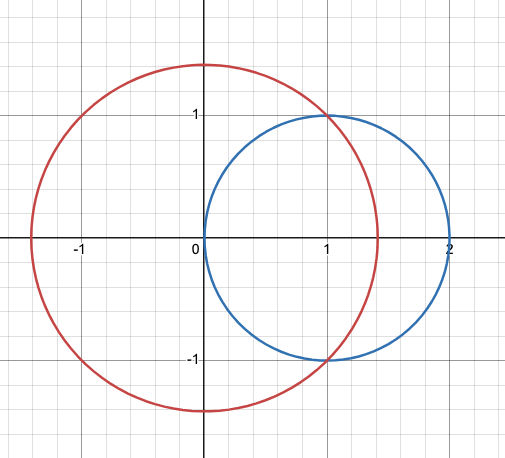
\includegraphics[width=\textwidth]{Image1}
\end{figure}
Next, we move them so that their intersection is at the origin. That is, we apply the function $f_1(z) = z - i -1$ to both of the circles, obtaining the below image:
\begin{figure}[H]
\centering
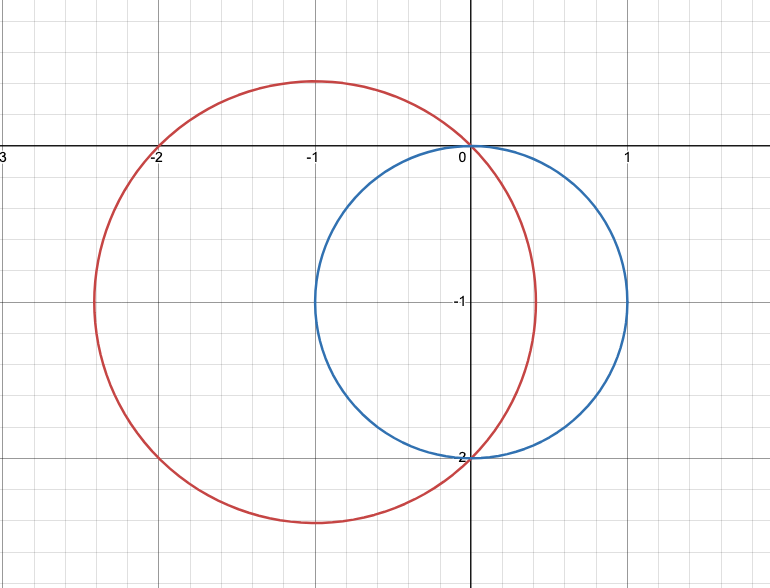
\includegraphics[width=\textwidth]{Image2}
\end{figure}
Next, we apply the mapping $f_2(z) = 1/z$. Since $f_2$ is a mobius transformation and $f_2(0) = \infty$, we know that $f_2$ sends both circles to lines. We first examine the effect of $1/z$ on the red circle. In particular, we compute $f_2(-2i) = i/2$ and $f_2(-2) = -1/2$. Computing the line between these two points yields $y = x + 1/2$. Thus the red circle is sent to the line $y = x+1/2$. Next, we examine the effect of $1/z$ on the blue circle. In particular, we compute $f_2(1-i)=(1+i)/2$ and $f_2(-1-i) = -1/2+i/2$. The line between these two points is $y = 1/2$. Thus the blue circle is sent to the line $y= 1/2$. Finally, we would like to determine where the region between these two circles goes. We compute $f_2(-i) = i$. Thus, we obtain the following image:
\begin{figure}[H]
\centering
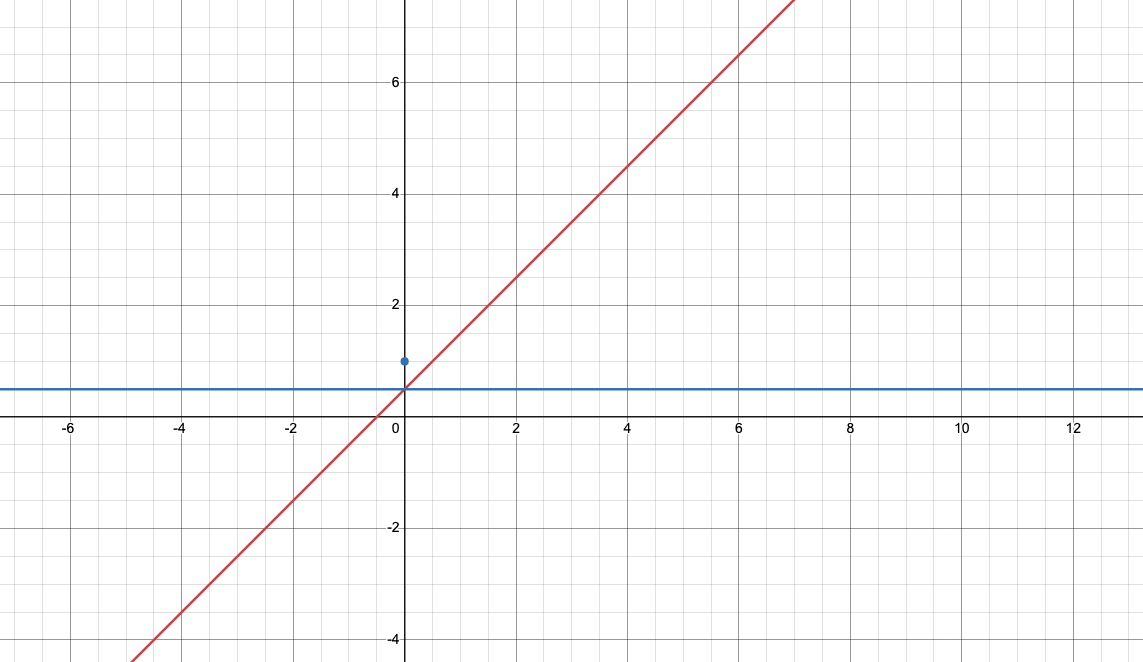
\includegraphics[width=\textwidth]{Image3}
\end{figure}
Next, we apply the mapping $f_3(z) = z - i/2$ to obtain the following image:
\begin{figure}[H]
\centering
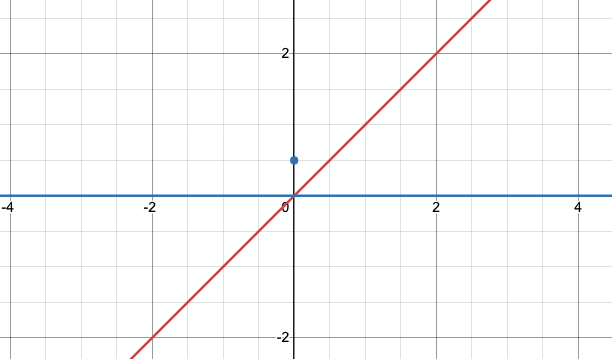
\includegraphics[width=\textwidth]{Image4}
\end{figure}
Now, we can apply the mapping $f_4(z) = e^{-i\pi/4}z$ to obtain the following image:
\begin{figure}[H]
\centering
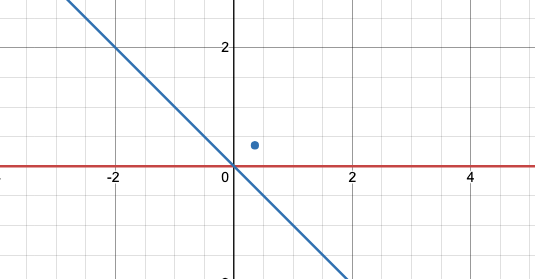
\includegraphics[width=\textwidth]{Image5}
\end{figure}
Next, we can apply the mapping $f_5(z) = z^{4/3}$ so that the region with the point in it is mapped to the upper half plane. Finally, we can apply the mapping $f_6(z) = (i-z)/(i+z)$ to ensure that the upper half-plane is mapped to the unit disk. Thus we find that $f_6\circ f_5 \circ f_4 \circ f_3 \circ f_2 \circ f_1$ is the desired conformal mapping.
\newpage
\subsection*{Problem 5}
First, we apply the mapping $f_1(z) = z - \frac{1}{2}i$ to the  strip $S_1 = \{z : \re z > 0, 0 < \imag z < 1\}$ to obtain the strip $S_2 = \{z : \re z > 0, -1/2 < \imag z < 1/2\}$. Then, we apply the mapping $f_2(z) = iz$ to the strip $S_2$ to obtain the strip $S_3 = \{z : -1/2 < \re z < 1/2, \imag z > 0\}$. Then, we apply the mapping $f_3(z) = \pi z$ to the strip $S_3$ to obtain the strip $S_4 = \{z : -\pi/2< \re z < \pi/2, \imag z > 0\}$. Next, we can apply the mapping $f_4(z) = \sin z$ to $S_4$ to obtain the upper half plane. Finally, we can apply the mapping $f_5(z) = (z-i)/(z+i)$ to the upper half plane to obtain the unit disk.
\end{document} 